% !TEX encoding = UTF-8
% !TEX TS-program = pdflatex
% !TEX root = ../tesi.tex

%**************************************************************
\chapter{Analisi dei requisiti}
\label{cap:analisi-requisiti}
%**************************************************************

Questo capitolo descrive i casi d'uso e i requisiti della piattaforma moviORDER, individuati e classificati per definire nel dettaglio obiettivi e funzionalità del sistema. I casi d'uso e i requisiti sono stati dedotti da un'analisi preliminare eseguita dal tutor aziendale, la quale è stata perfezionata dallo stagista per perseguire massima efficienza ed efficacia del sistema. Le convenzioni adottate per la stesura di casi d'uso e requisiti sono presenti in Appendice §\ref{}.

\section{Casi d'uso}

Per lo studio dei casi di utilizzo della piattaforma, si sono utilizzati i diagrammi dei casi d'uso che meglio descrivono funzioni e/o servizi offerti dal sistema, così come sono percepiti e utilizzati dagli attori che interagiscono con il sistema stesso. Per la definizione dei diagrammi UML dei casi d’uso, viene utilizzato lo standard UML 2.0.

\subsection{Dominio}

Lo scopo di moviORDER è permettere alle aziende che forniscono dei prodotti di vendere gli stessi ai propri clienti tramite un'applicazione multipiattaforma. Quindi moviORDER viene distribuita da VISIONEIMPRESA alle aziende che forniscono prodotti, la quale viene distribuita dalle aziende stesse ai propri clienti. Gli utilizzatori finali di moviORDER sono quindi i clienti delle singole aziende clienti di VISIONEIMPRESA.
L'accesso all'applicazione è consentito solamente agli utenti provvisti di credenziali di accesso, le quali vengono distribuite, insieme all'applicazione, dal fornitore. Non è prevista quindi una funzionalità di registrazione. Nel contesto di moviORDER vi sono quindi due tipologie di attori:
\begin{enumerate}
	\item \textbf{Utente non autenticato}: è un utente in possesso dell'applicazione al quale viene offerta la sola funzionalità di autenticazione. Una volta che un utente non autenticato accede a moviORDER diventa un utente autenticato;
	\item \textbf{Utente autenticato}: è un utente che è riuscito ad accedere al sistema e che può usufruire di tutte le sue funzionalità. Tra le funzionalità offerte all'utente autenticato vi sono:
	\begin{itemize}
		\item possibilità di effettuare il logout;
		\item possibilità di aggiungere articoli al proprio carrello;
		\item possibilità di modificare gli articoli nel proprio carrello;
		\item possibilità di rimuovere articoli dal proprio carrello;
		\item possibilità di inviare un ordine alla propria azienda.
	\end{itemize}
\end{enumerate}

\subsection{Visione generale}

In questa sezione vengono presentati i casi d'uso generali della piattaforma moviORDER.

\subsubsection{Caso d'uso generale - Utente non autenticato}

Nella figura \ref{fig:altoLivello1} è mostrata la visione generale concernente l'utente non ancota riconosciuto dal sistema.

\begin{figure}[!h] 
    \centering 
    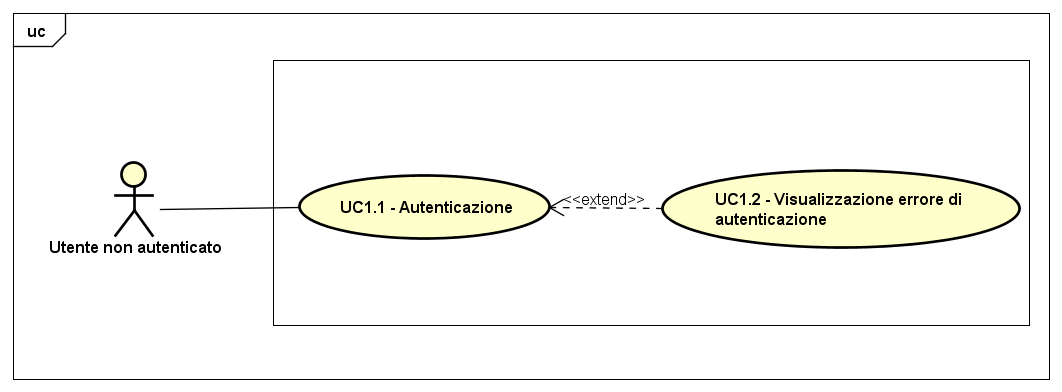
\includegraphics[width=0.9\columnwidth]{usecase/generaleNonAutenticato} 
    \caption{Diagramma ad alto livello 1 - Utente non autenticato}
    \label{fig:altoLivello1}
\end{figure}

\begin{itemize}
	\item \textbf{Attore}: Utente non autenticato;
	\item \textbf{Descrizione}: L'attore può accedere al portale (UC1);
	\item \textbf{Pre-condizioni}: L'attore si trova nella pagina di autenticazione di moviORDER e possiede le credenziali di accesso;
	\item \textbf{Post-condizioni}: Il sistema permette all'utente di autenticarsi;
	\item \textbf{Scenario principale}: Utilizzo della funzionalità di autenticazione (UC1);
	\item \textbf{Estensione}: Errore nel tentativo di accesso a moviORDER (UC2).
\end{itemize}

\newpage

\subsubsection{Caso d'uso generale - Utente autenticato}

Nella figura \ref{fig:altoLivello2} è mostrata la visione generale concernente l'utente riconosciuto dal sistema.

\begin{figure}[!h] 
    \centering 
    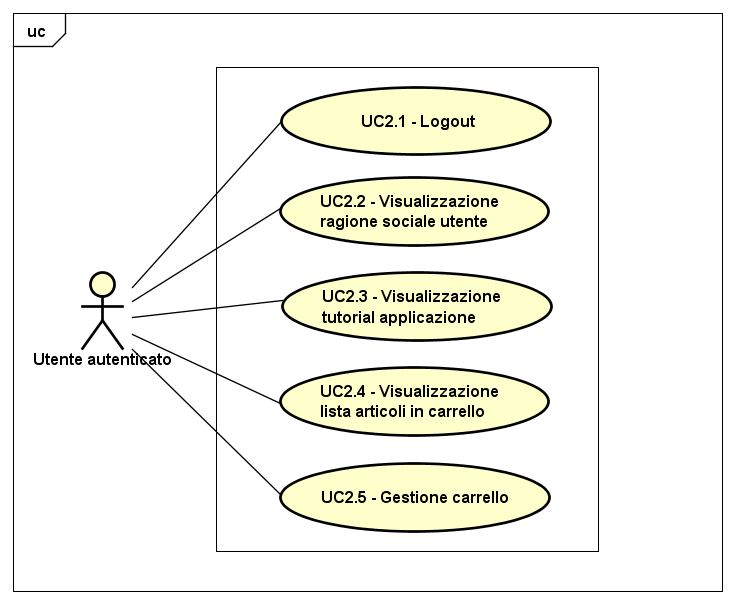
\includegraphics[width=0.9\columnwidth]{usecase/generaleAutenticato} 
    \caption{Diagramma ad alto livello 2 - Utente autenticato}
    \label{fig:altoLivello2}
\end{figure}

\begin{itemize}
	\item \textbf{Attore}: Utente autenticato;
	\item \textbf{Descrizione}: L'attore può usufruire delle funzionalità offerte dal sistema;
	\item \textbf{Pre-condizioni}: L'attore è stato riconosciuto dal sistema;
	\item \textbf{Post-condizioni}: Il sistema permette all'utente di utilizzare le funzionalità;
	\item \textbf{Scenario principale}: 
		\begin{enumerate}
			\item Logout (UC3);
			\item Visualizzazione della ragione sociale (UC4);
			\item Visualizzazione del tutorial dell'applicazione (UC5);
			\item Visualizzazione della lista degli articoli in carrello (UC6);
			\item Gestione del carrello (UC7).
		\end{enumerate}
\end{itemize}

\newpage

\subsection{Dettaglio dei casi d'uso}


\section{Tracciamento dei requisiti}

Da un'attenta analisi dei requisiti e degli use case effettuata sul progetto è stata stilata la tabella che traccia i requisiti in rapporto agli use case.\\
Sono stati individuati diversi tipi di requisiti e si è quindi fatto utilizzo di un codice identificativo per distinguerli.\\
Il codice dei requisiti è così strutturato R(F/Q/V)(N/D/O) dove:
\begin{enumerate}
	\item[R =] requisito
    \item[F =] funzionale
    \item[Q =] qualitativo
    \item[V =] di vincolo
    \item[N =] obbligatorio (necessario)
    \item[D =] desiderabile
    \item[Z =] opzionale
\end{enumerate}
Nelle tabelle \ref{tab:requisiti-funzionali}, \ref{tab:requisiti-qualitativi} e \ref{tab:requisiti-vincolo} sono riassunti i requisiti e il loro tracciamento con gli use case delineati in fase di analisi.

\newpage

\begin{table}%
\caption{Tabella del tracciamento dei requisti funzionali}
\label{tab:requisiti-funzionali}
\begin{tabularx}{\textwidth}{lXl}
\hline\hline
\textbf{Requisito} & \textbf{Descrizione} & \textbf{Use Case}\\
\hline
RFN-1     & L'interfaccia permette di configurare il tipo di sonde del test & UC1 \\
\hline
\end{tabularx}
\end{table}%

\begin{table}%
\caption{Tabella del tracciamento dei requisiti qualitativi}
\label{tab:requisiti-qualitativi}
\begin{tabularx}{\textwidth}{lXl}
\hline\hline
\textbf{Requisito} & \textbf{Descrizione} & \textbf{Use Case}\\
\hline
RQD-1    & Le prestazioni del simulatore hardware deve garantire la giusta esecuzione dei test e non la generazione di falsi negativi & - \\
\hline
\end{tabularx}
\end{table}%

\begin{table}%
\caption{Tabella del tracciamento dei requisiti di vincolo}
\label{tab:requisiti-vincolo}
\begin{tabularx}{\textwidth}{lXl}
\hline\hline
\textbf{Requisito} & \textbf{Descrizione} & \textbf{Use Case}\\
\hline
RVO-1    & La libreria per l'esecuzione dei test automatici deve essere riutilizzabile & - \\
\hline
\end{tabularx}
\end{table}%